\mfpicnumber{1}

\opengraphsfile{PowerEqIneq}

\setcounter{footnote}{0}

\label{PowerEqIneq}

In this section, we set about solving equations and inequalities involving power functions.  Our first example demonstrates the usual sorts of strategies to employ when solving equations.

\begin{ex} \label{powerequationex}  Solve the following equations analytically and verify your answers using a graphing utility.


\begin{multicols}{2}
\begin{enumerate}

\item \label{first} $(7-x)^{\frac{3}{2}} = 8$ 
\item \label{second} $(2t-1)^{\frac{2}{3}} -4 = 0$

\setcounter{HW}{\value{enumi}}
\end{enumerate}
\end{multicols}

\begin{multicols}{2}
\begin{enumerate}
\setcounter{enumi}{\value{HW}}

\item $(x+3)^{0.5} = 2(7-x)^{0.5}+1$ 
\item $2t^{\frac{2}{3}} + 5t^{\frac{1}{3}} = 3$

\setcounter{HW}{\value{enumi}}
\end{enumerate}
\end{multicols}


\begin{multicols}{2}
\begin{enumerate}
\setcounter{enumi}{\value{HW}}

\item $2(3x-1)^{-0.5}  = 3x (3x-1)^{-1.5}$ 
\item $6(9-t^2)^{\frac{1}{3}} = 4t^2 (9-t^2)^{-\frac{2}{3}}$

\setcounter{HW}{\value{enumi}}
\end{enumerate}
\end{multicols}

{\bf Solution.}

\begin{enumerate}

\item  One way to proceed to solve  $(7-x)^{\frac{3}{2}} = 8$ is to use Definition \ref{rationalexponentdefna} to rewrite $(7-x)^{\frac{3}{2}}$ as either $(\sqrt{7-x})^3$ or $\sqrt{(7-x)^3}$.  We opt for the former since, thinking ahead,  $8$ is a perfect cube: 

\[ \begin{array}{rclr}

(7-x)^{\frac{3}{2}} & = & 8 & \\

(\sqrt{7-x})^3 & = & 8 & \text{rewrite using Definition \ref{rationalexponentdefna}} \\

\sqrt[3]{(\sqrt{7-x})^3} & = & \sqrt[3]{8} & \text{extract cube roots}  \\

\sqrt{7-x} & = & 2 & \text{$\sqrt[3]{u^3}= u$} \\ \end{array} \]

From $\sqrt{7-x} =  2$, we square both sides and obtain $7-x = 4$, so $x = 3$.  We verify our answer analytically by substituting $x=3$ into the original equation and it checks.

Geometrically, we are looking for where the graph of $f(x) = (7-x)^{\frac{3}{2}}$ intersects the graph of $g(x) = 8$.  While we could sketch both curves by hand and gauge the reasonableness of the result,\footnote{consider this an exercise!} we are instructed to use a graphing utility.  Below on the left and see the intersection point of both graphs is $(3,8)$, thereby checking our solution $x = 3$.

\item  Proceeding similarly to the above, to solve $(2t-1)^{\frac{2}{3}} -4 = 0$, we rewrite $(2t-1)^{\frac{2}{3}}$ as $(\sqrt[3]{2t-1})^2$ and solve:

\[ \begin{array}{rclr}
(2t-1)^{\frac{2}{3}} -4  & = & 0 & \\

(\sqrt[3]{2t-1})^2 - 4 & = & 0 & \text{rewrite using Definition \ref{rationalexponentdefna}} \\
(\sqrt[3]{2t-1})^2 & = & 4 & \text{isolate the variable term} \\

\sqrt{(\sqrt[3]{2t-1})^2 } & = & \sqrt{4} & \text{extract square roots} \\

|\sqrt[3]{2t-1}| & = & 2 & \text{$\sqrt{u^2} = |u|$} \\

\sqrt[3]{2t-1} & = & \pm 2 & \text{ for $c>0$, $|u| = c$ is equivalent to $u = \pm c$.} \end{array} \]

From $\sqrt[3]{2t-1}  = 2$ we cube both sides and obtain $2t-1 = 8$, so $t = \frac{9}{2} = 4.5$.  Similarly, from $\sqrt[3]{2t-1}  = -2$, we cube both sides and obtain $2t-1 = -8$, so $t = -\frac{7}{2} = -3.5$.  Both of these solutions check in the given equation.

In this case we are looking for where the graph of $f(t) = (2t-1)^{\frac{2}{3}} -4$ intersects the graph of $g(t) = 0$ - i.e., the $t$-intercepts of the graph of $g$.  We find these are $(-3.5,0)$ and $(4.5,0)$, as predicted.

\begin{center}

\begin{tabular}{cc}

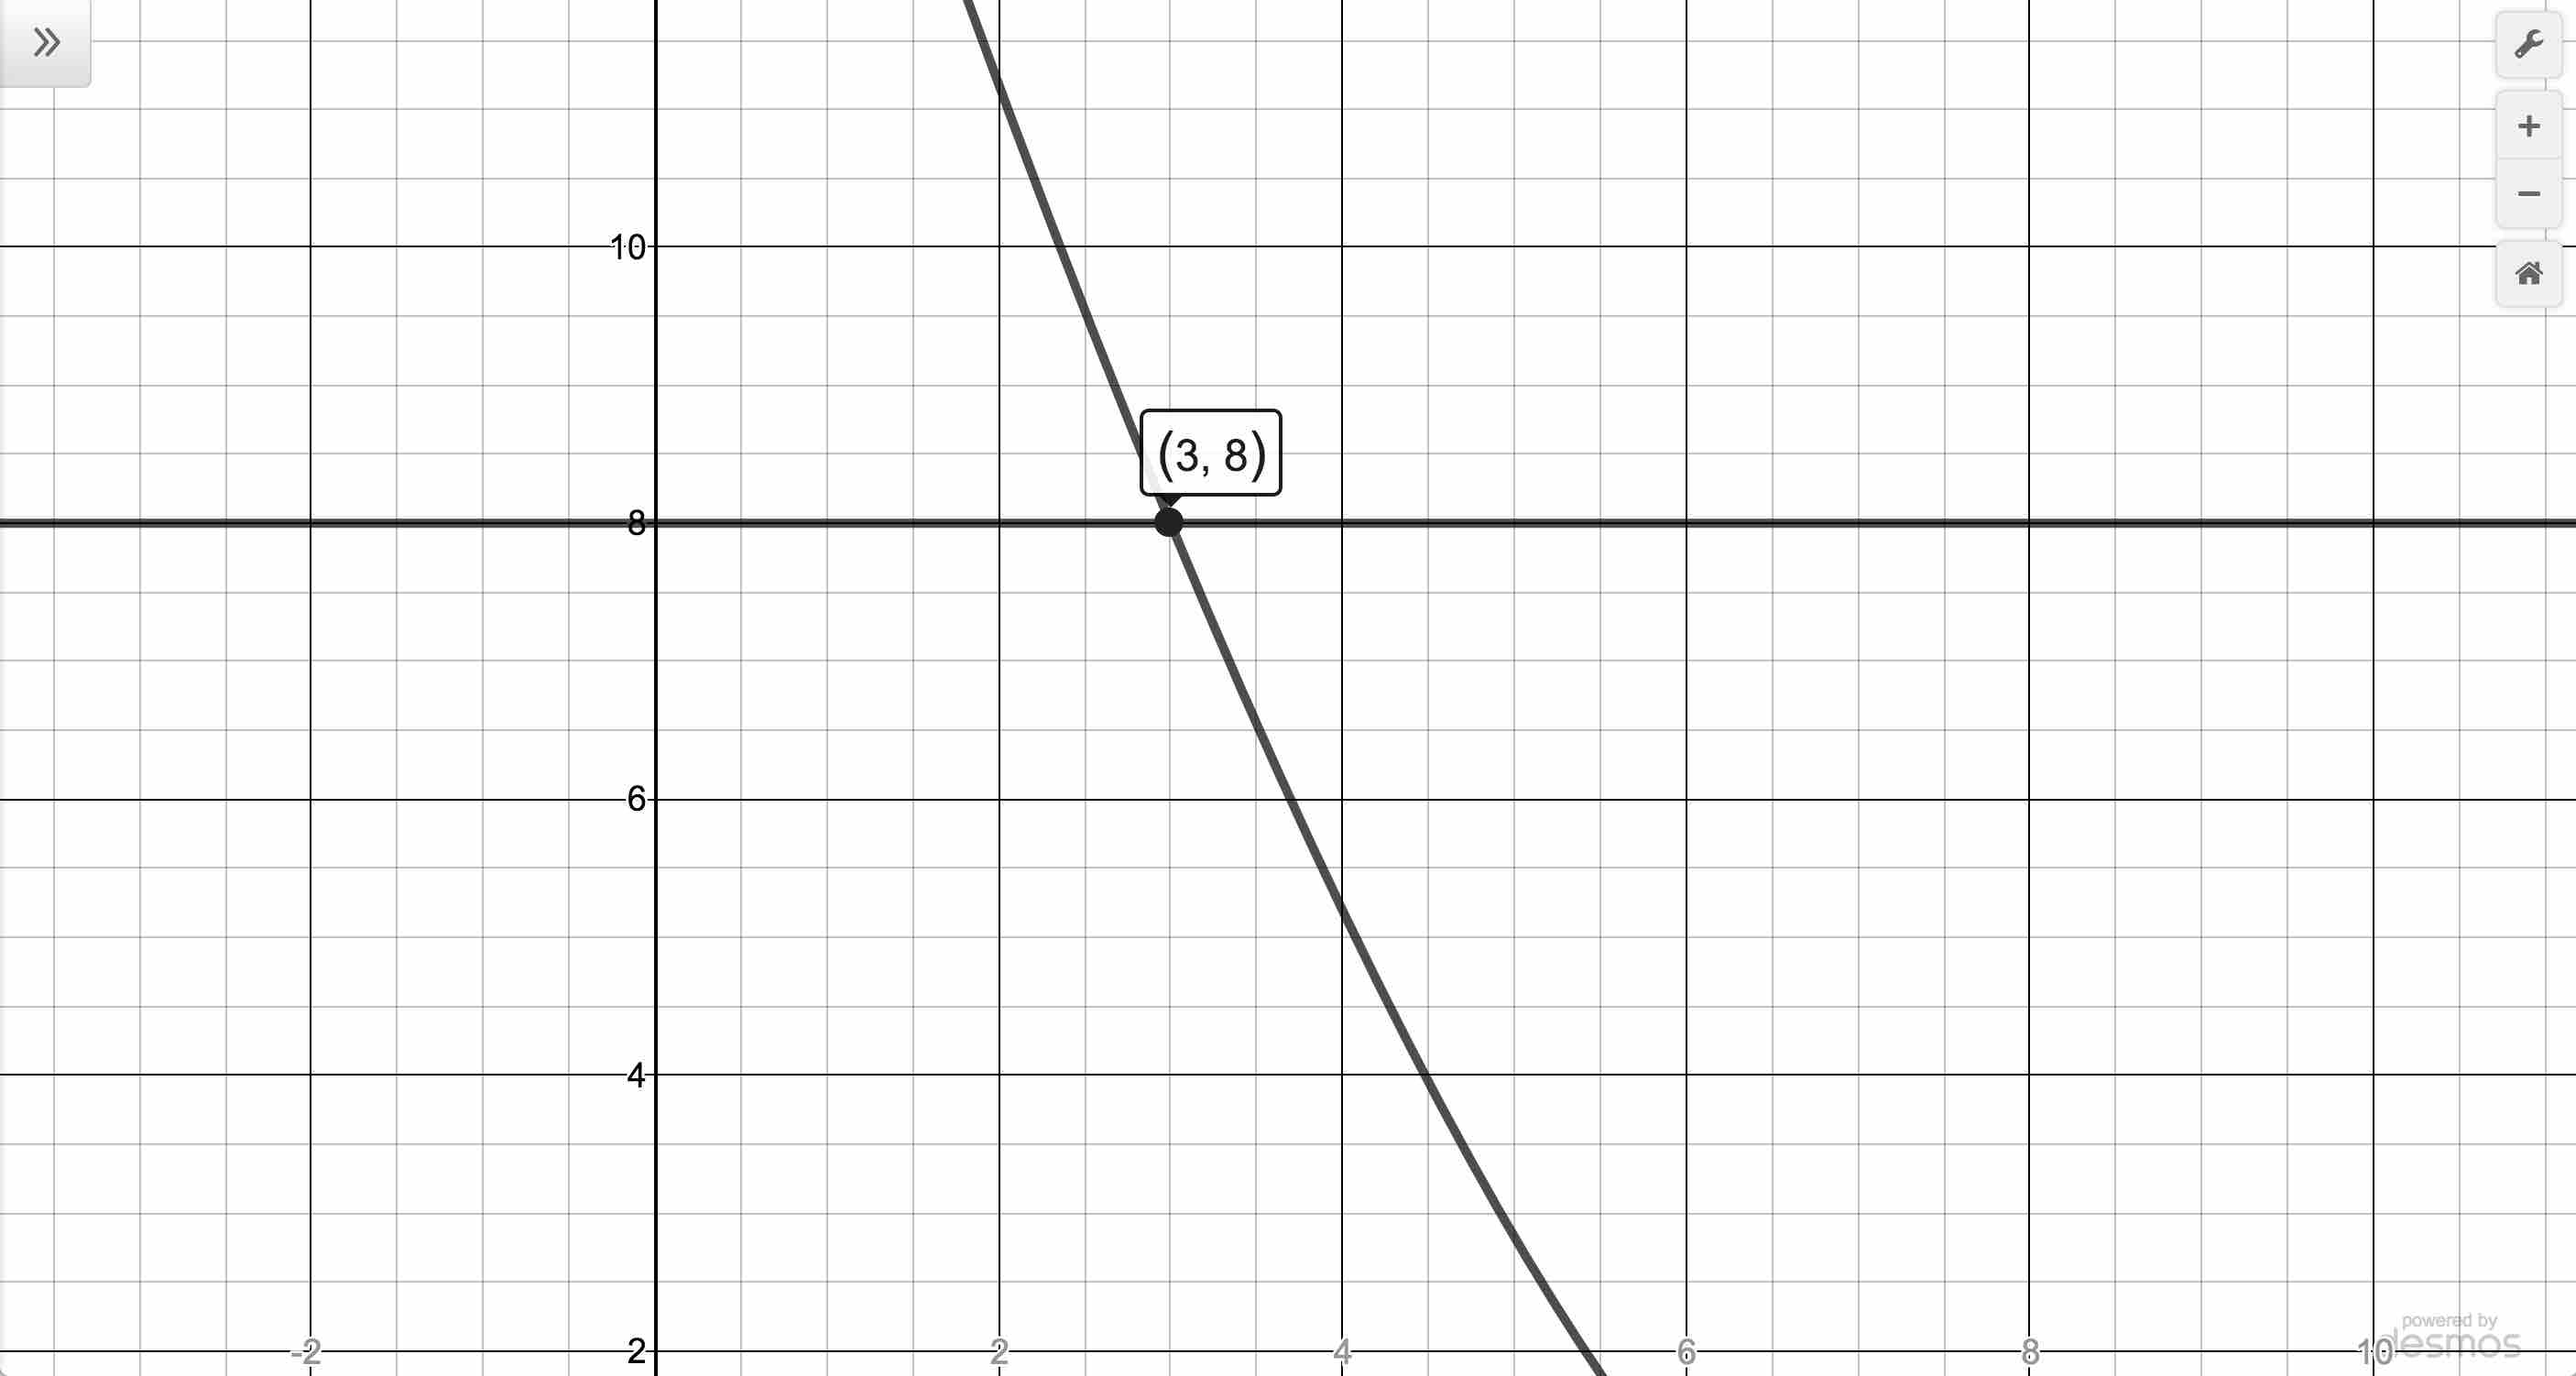
\includegraphics[width=3in]{./PowerEqIneqGraphics/PowerEqEx01.jpg} & 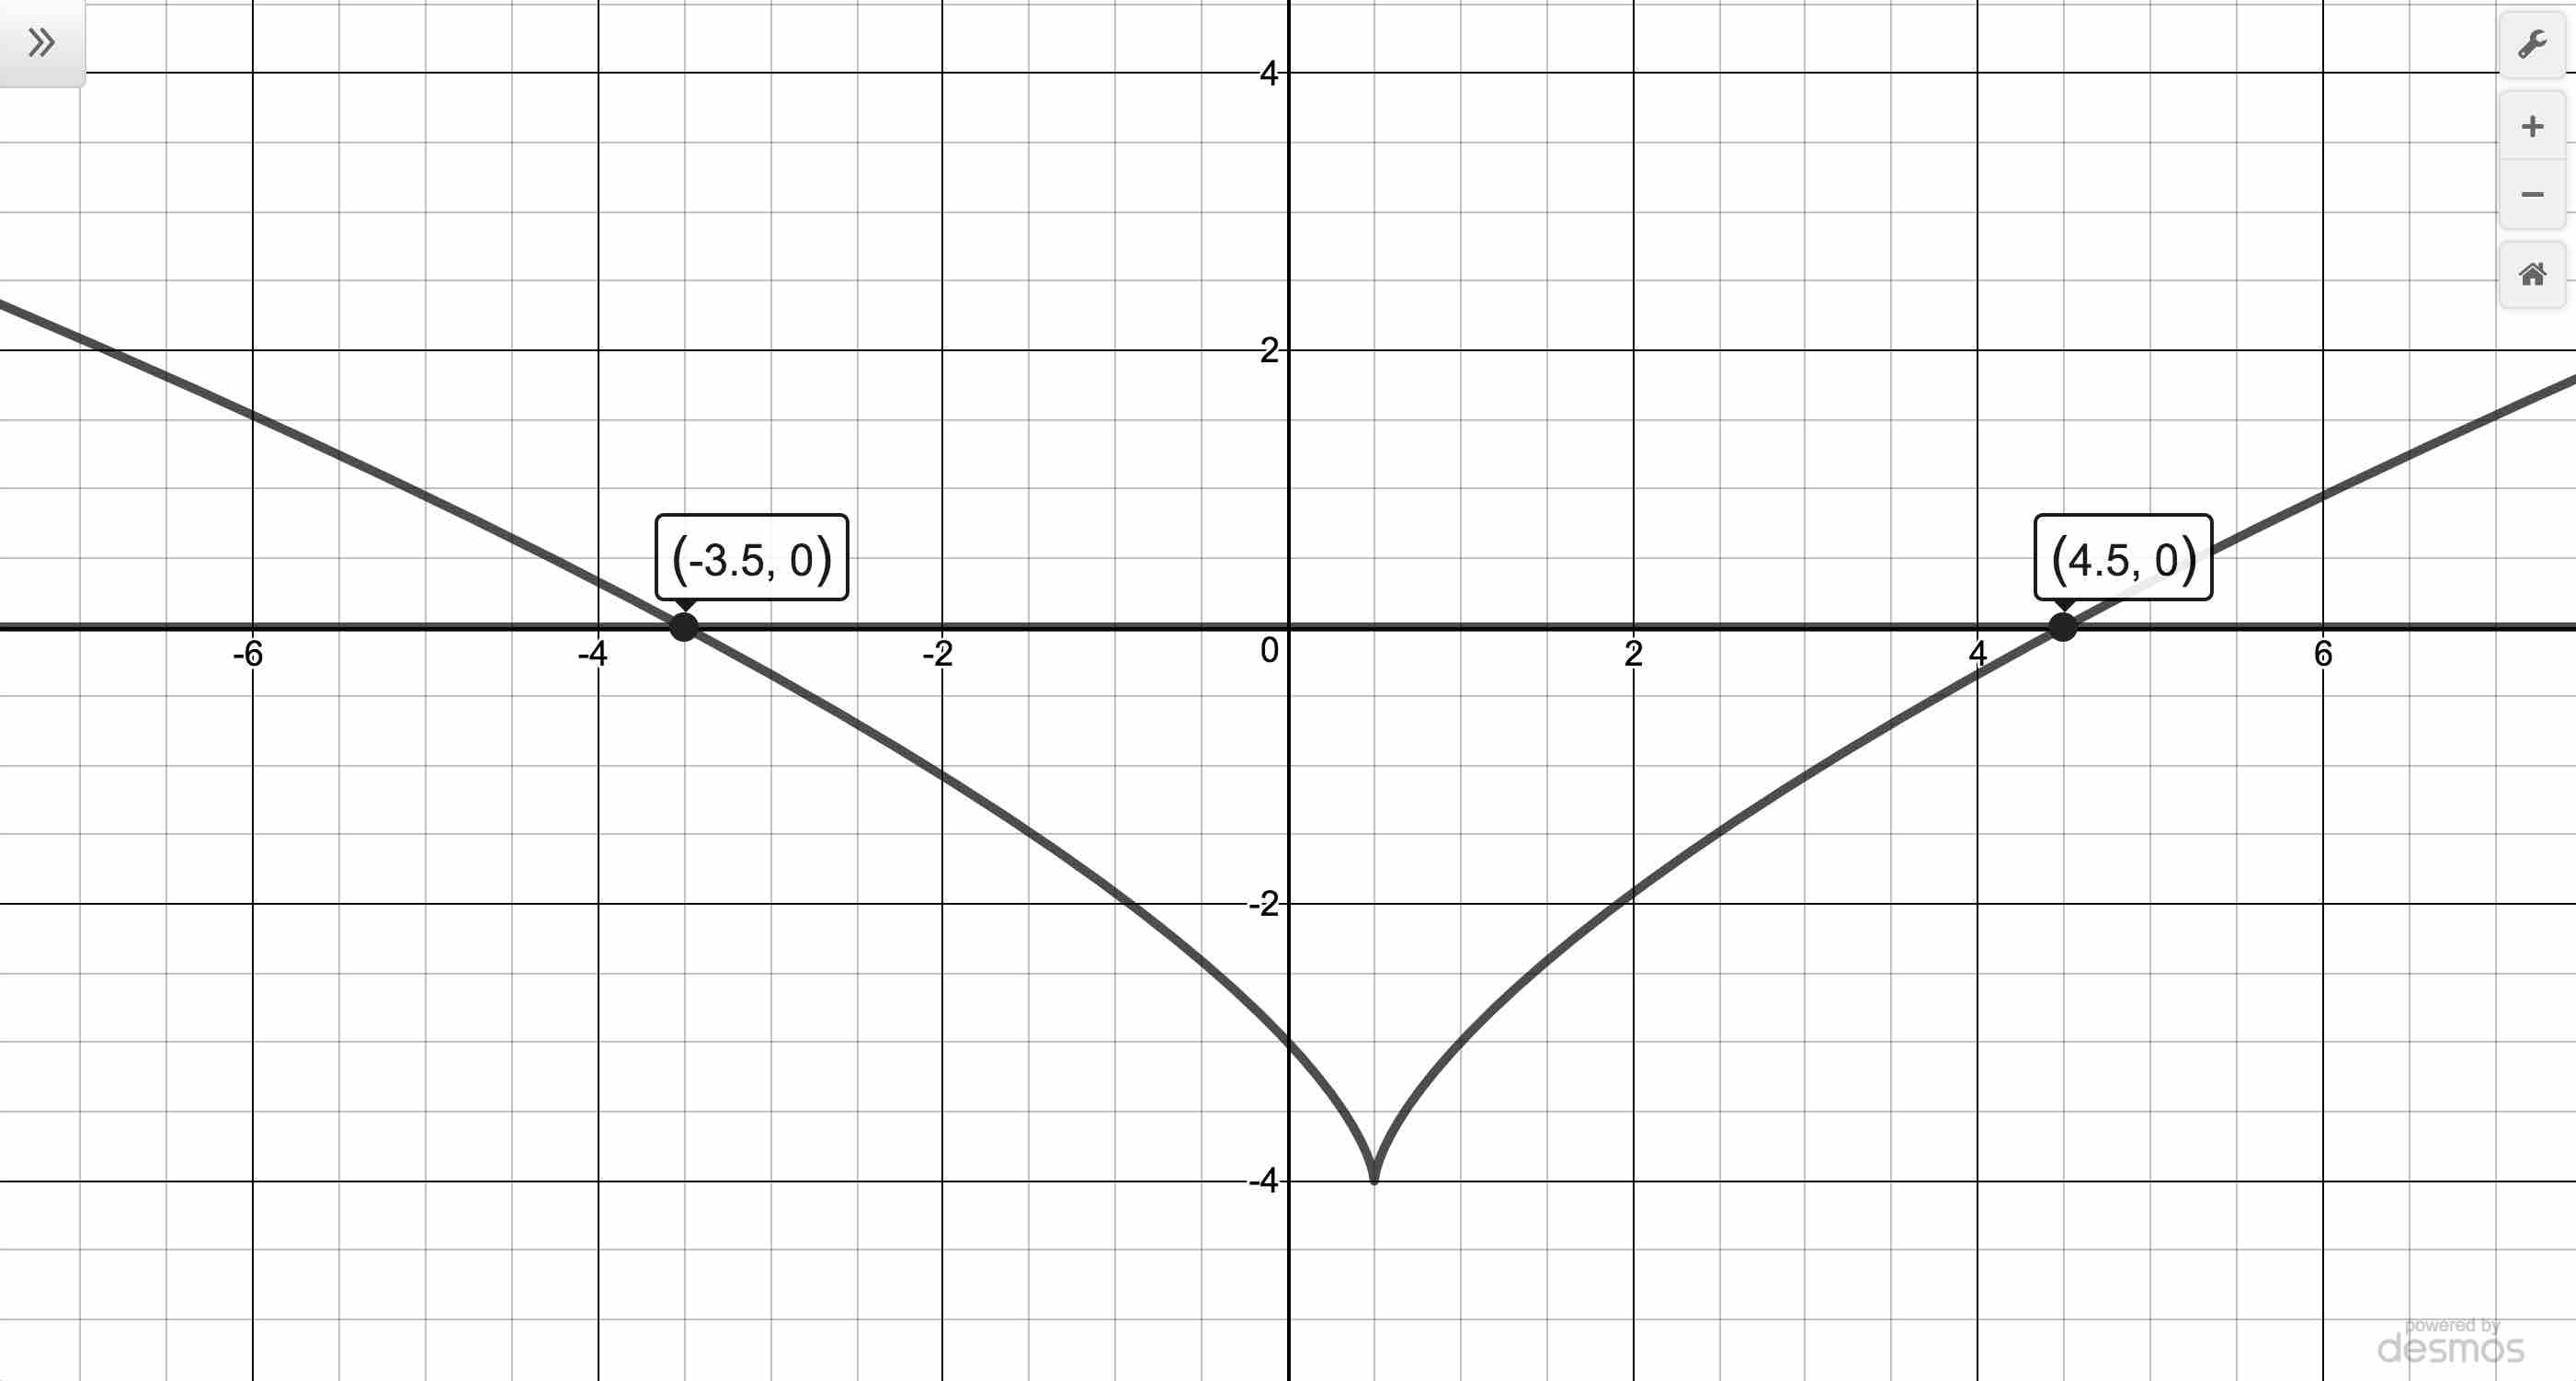
\includegraphics[width=3in]{./PowerEqIneqGraphics/PowerEqEx02.jpg} \\

Checking $(7-x)^{\frac{3}{2}} = 8$  & Checking  $(2t-1)^{\frac{2}{3}} -4 = 0$ \\

\end{tabular}

\end{center} 

\item Since $0.5 = \frac{1}{2}$, we may rewrite $(x+3)^{0.5} = 2(7-x)^{0.5}+1$ as  $(x+3)^{\frac{1}{2}} = 2(7-x)^{\frac{1}{2}}+1$.  Using Definition \ref{rationalexponentdefna}, we then have $\sqrt{x+3} = 2\sqrt{7-x} + 1$.  Since one of the square roots is already isolated, we can rid ourselves of it by squaring both sides.

\[ \begin{array}{rclr}

\sqrt{x+3} & = & 2\sqrt{7-x} + 1 & \\

 (\sqrt{x+3})^2 & = & (2\sqrt{7-x} + 1)^2 & \text{square both sides} \\
 
 x+3 & = & (2 \sqrt{7-x})^2 + 2 (2 \sqrt{7-x})(1) + 1 & \text{$(\sqrt{u})^2 = u$ and $(a+b)^2 = a^2 + 2ab +b^2$} \\

 
 x+3 & = & 4(7-x) + 4\sqrt{7-x} + 1 &  \text{$(ab)^2 = a^2b^2$ and, again, $(\sqrt{u})^2 = u$} \\
 
 x+3 & = & 28-4x+4\sqrt{7-x} + 1 & \\
 
 5x-26 & = & 4\sqrt{7-x} & \text{isolate $\sqrt{7-x}$} \\ \end{array} \]
 
We square both sides \textit{again} and get $(5x-26)^2 = (4\sqrt{7-x})^2$ which reduces to $25x^2-260x+676 = 16(7-x)$. At last, we have a quadratic equation which we can solve by setting to zero and factoring.  We get  $25x^2-244x+564 = 0$, so $(x-6)(25x-94) = 0$ so $x = 6$ or $x = \frac{94}{25} = 3.76$.  When we go to check these answers, we find $x=6$ does check, but $x = 3.76$ does not. Hence, $x=3.76$ is an `extraneous' solution.\footnote{We invite the reader to see at which point in our machinations $x=3.76$ \textit{does} check.  Knowing a solution is extraneous is one thing;  understanding \textit{how} it came about is another.}

We graph both $f(x) = \sqrt{x+3}$ and $g(x) = 2\sqrt{7-x} + 1$ below (once again, we could graph these by hand!) and confirm there is only one intersection point, $(6,3)$.

\item  While we \textit{could} approach solving  $2t^{\frac{2}{3}} + 5t^{\frac{1}{3}} = 3$ as the previous example, we would encounter cubing binomials\footnote{that is, expanding things like $(a+b)^3$.} which we would prefer to avoid.  Instead, we take a step back and notice there are three terms here with the exponent on one term exactly twice the exponent on another term.  We have ourselves a `quadratic in disguise.'\footnote{See Section \ref{AppQuadEqus} or, more recently, Example \ref{polyquadinform} in Section \ref{RealZeros}.} To help us see the forest for the trees, we let $u = t^{\frac{1}{3}}$ so that $u^2 = t^{\frac{2}{3}}$. (Note that since root here, $3$, is odd, we can use the properties of exponents stated in Theorem \ref{exponentprops}.)  Hence, in terms of $u$, the equation   $2t^{\frac{2}{3}} + 5t^{\frac{1}{3}} = 3$ becomes the quadratic $2u^2 + 5u = 3$, or $2u^2 + 5u - 3 = 0$.  Factoring gives $(2u-1)(u+3) = 0$ so $u = t^{\frac{1}{3}} = \frac{1}{2}$ or $u = t^{\frac{1}{3}} = -3$.  Since $t^{\frac{1}{3}} = \sqrt[3]{t}$, we solve both equations by cubing both sides to get $t = \frac{1}{8} = 0.125$ and $t = -27$.  Both of these solutions check in our original equation.  Looking at the graphs of $f(t) = 2t^{\frac{2}{3}} + 5t^{\frac{1}{3}}$ and $g(t) = 3$, we find two intersection points, $(-27,3)$ and $(0.125,3)$, as required.

\begin{center}

\begin{tabular}{cc}

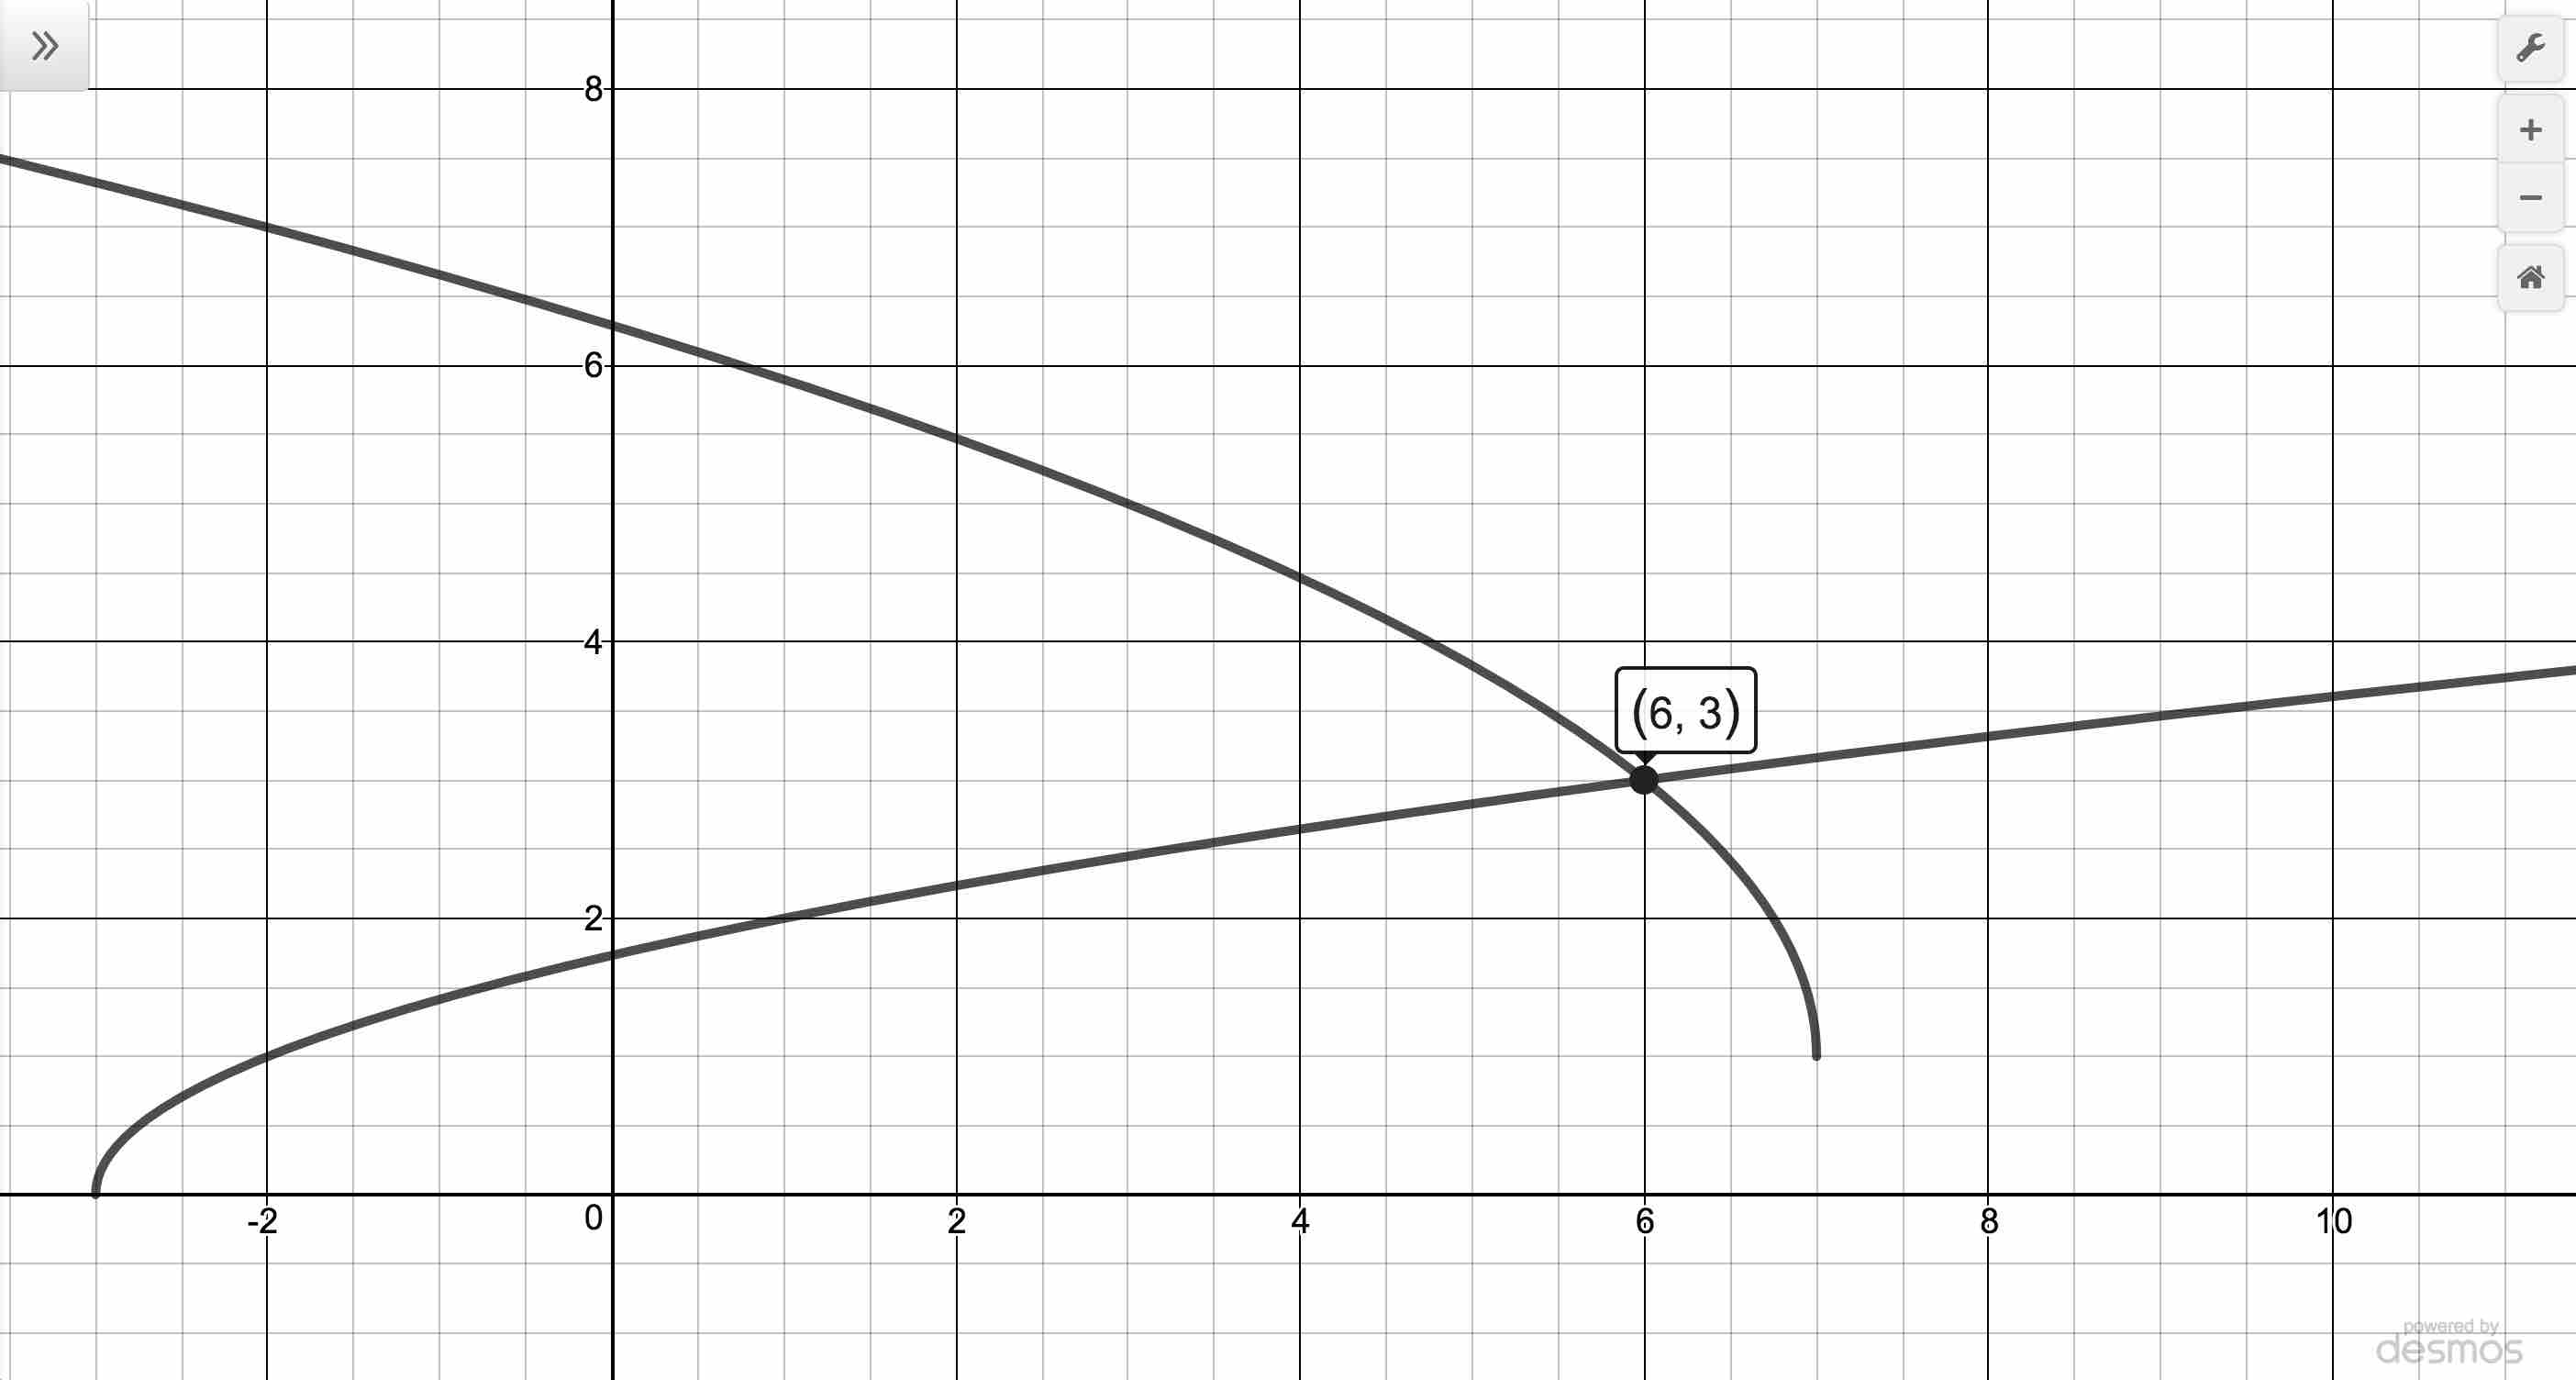
\includegraphics[width=3in]{./PowerEqIneqGraphics/PowerEqEx03.jpg} & 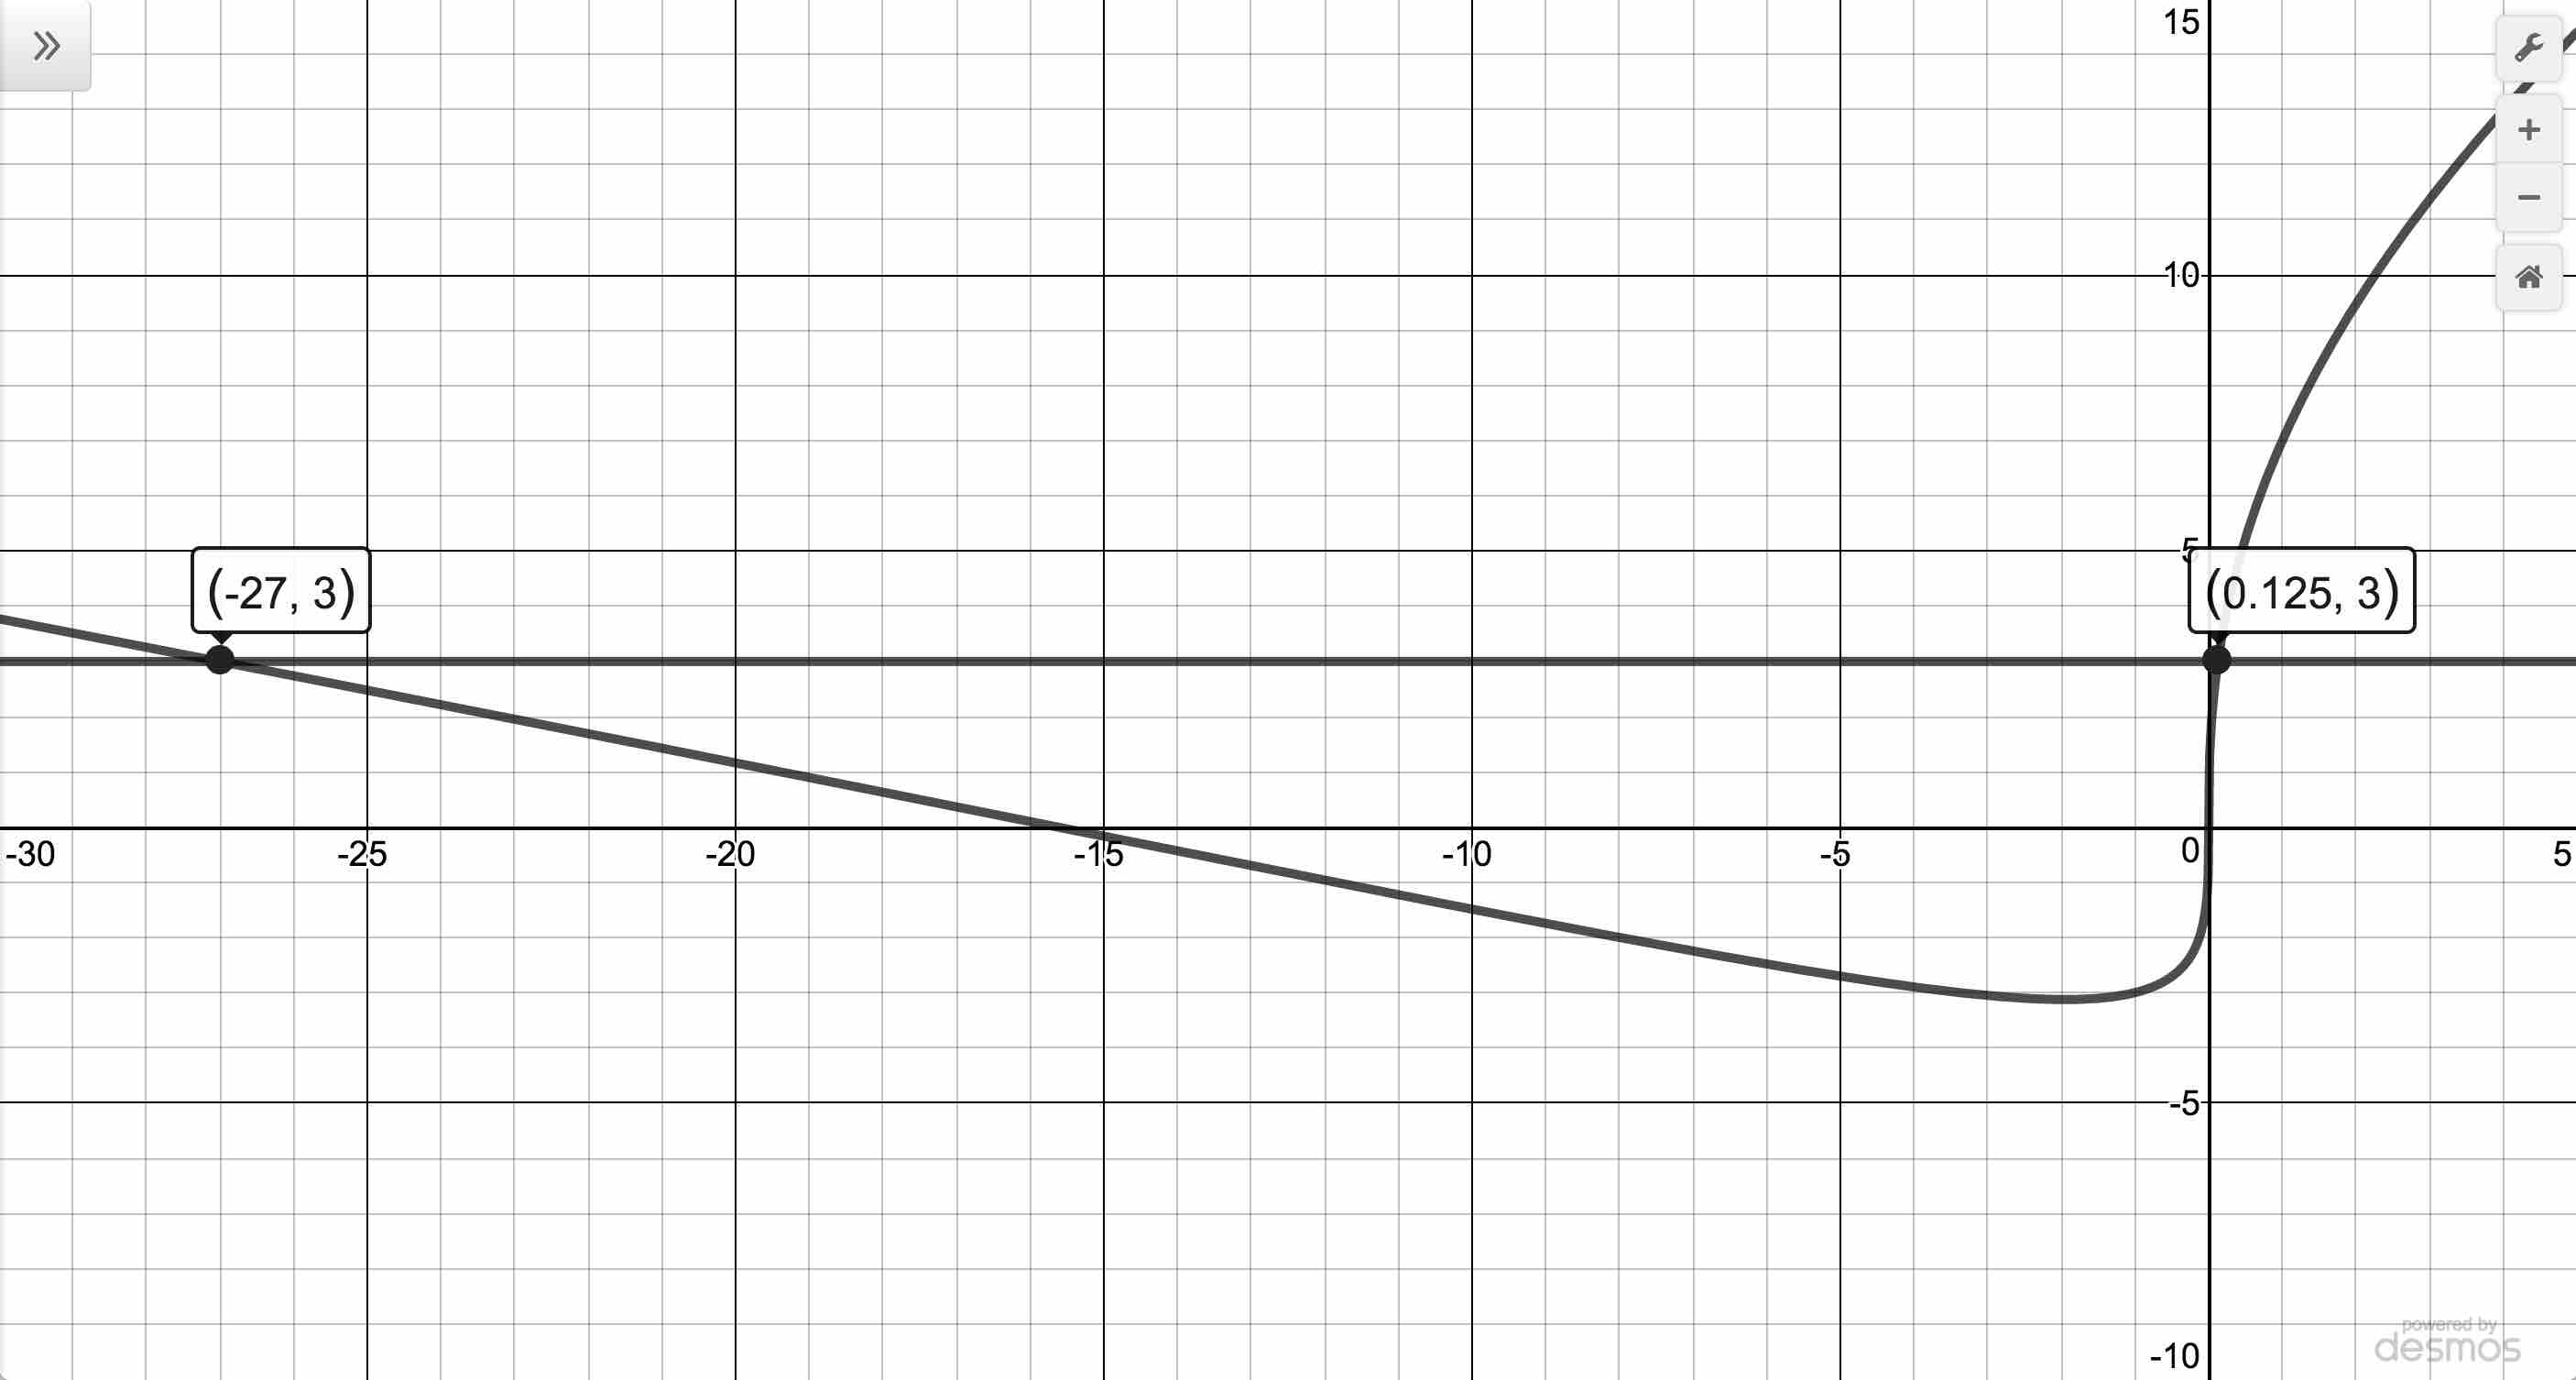
\includegraphics[width=3in]{./PowerEqIneqGraphics/PowerEqEx04.jpg} \\

Checking $(x+3)^{0.5} = 2(7-x)^{0.5}+1$ & Checking  $2t^{\frac{2}{3}} + 5t^{\frac{1}{3}} = 3$ \\

\end{tabular}

\end{center} 


\item Next we are to solve $2(3x-1)^{-0.5}  = 3x (3x-1)^{-1.5}$ which, when written without negative exponents is: $\frac{2}{(3x-1)^{0.5}} = \frac{3x}{(3x-1)^{1.5}}$.  Since the rational exponents here are $0.5 = \frac{1}{2}$ and $1.5 = \frac{3}{2}$, both involve an \textit{even} indexed root (the square root in this case!) which means $3x-1 \geq 0$.  Moreover, since the $3x-1$ resides in the \textit{denominator} $3x - 1 \neq 0$ so our equation is really valid only for values of $x$ where $3x-1>0$ or $x > \frac{1}{3}$.  Hence, we clear denominators and can apply Theorem \ref{exponentprops}:

\[ \begin{array}{rclr}

\dfrac{2}{(3x-1)^{0.5}} & = & \dfrac{3x}{(3x-1)^{1.5}} & \\

\left[ \dfrac{2}{(3x-1)^{0.5}} \right] \cdot (3x-1)^{1.5} & = & \left[  \dfrac{3x}{(3x-1)^{1.5}} \right ] \cdot (3x-1)^{1.5} & \\

2 \cdot \dfrac{(3x-1)^{1.5}}{(3x-1)^{0.5}} & = & 3x & \\

2 (3x-1)^{1.5-0.5} & = & 3x & \text{Theorem \ref{exponentprops} applies since $3x-1 > 0$.} \\

2 (3x-1)^{1} & = & 3x & \\  \end{array} \]

We get $6x-2 = 3x$, or $x = \frac{2}{3}$.  Since $x = \frac{2}{3} > \frac{1}{3}$, we keep it and, sure enough, it  checks in our original equation. Graphically we see $f(x)=2(3x-1)^{-0.5}$ intersects $g(x) = 3x (3x-1)^{-1.5}$ at the point $(0.6667, 2)$ which is the graphing utility's way of representing $\left(\frac{2}{3}, 2\right)$.

\item  Our last equation to solve is $6(9-t^2)^{\frac{1}{3}} = 4t^2 (9-t^2)^{-\frac{2}{3}}$, which, when rewritten without negative exponents is: $6(9-t^2)^{\frac{1}{3}} = \frac{4t^2}{(9-t^2)^{\frac{2}{3}}}$  .   Again, the root here ($3$) is odd, so we can use the exponent properties listed in Theorem \ref{exponentprops}.   We begin by clearing denominators: 


\[ \begin{array}{rclr}

6(9-t^2)^{\frac{1}{3}} & = & \frac{4t^2}{(9-t^2)^{\frac{2}{3}}} & \\

6(9-t^2)^{\frac{1}{3}} \cdot (9-t^2)^{\frac{2}{3}} & = & \left[   \frac{4t^2}{(9-t^2)^{\frac{2}{3}}}  \right ] \cdot (9-t^2)^{\frac{2}{3}} & \\

6(9-t^2)^{\frac{1}{3} + \frac{2}{3}}& = & 4t^2 &  \text{Theorem \ref{exponentprops} applies since the root here $3$ is odd.} \\

6(9-t^2)^{1} & = & 4t^2 &\\   \end{array} \]

We get $54 - 6t^2 = 4t^2$ or $10t^2 = 54$.  As fraction $t^2 = \frac{54}{10} = \frac{27}{5}$ so $t = \pm \sqrt{\frac{27}{5}} = \pm 3 \sqrt{15}{5}$.  While not the easiest to check analytically, both of these solutions do work in the original equation.  Graphing $f(t) = 6(9-t^2)^{\frac{1}{3}} $ and $g(t) =  4t^2 (9-t^2)^{-\frac{2}{3}}$ below, we see the graphs intersect when $t \approx \pm 2.324$ which are decimal approximations of our exact answers.

\begin{center}

\begin{tabular}{cc}

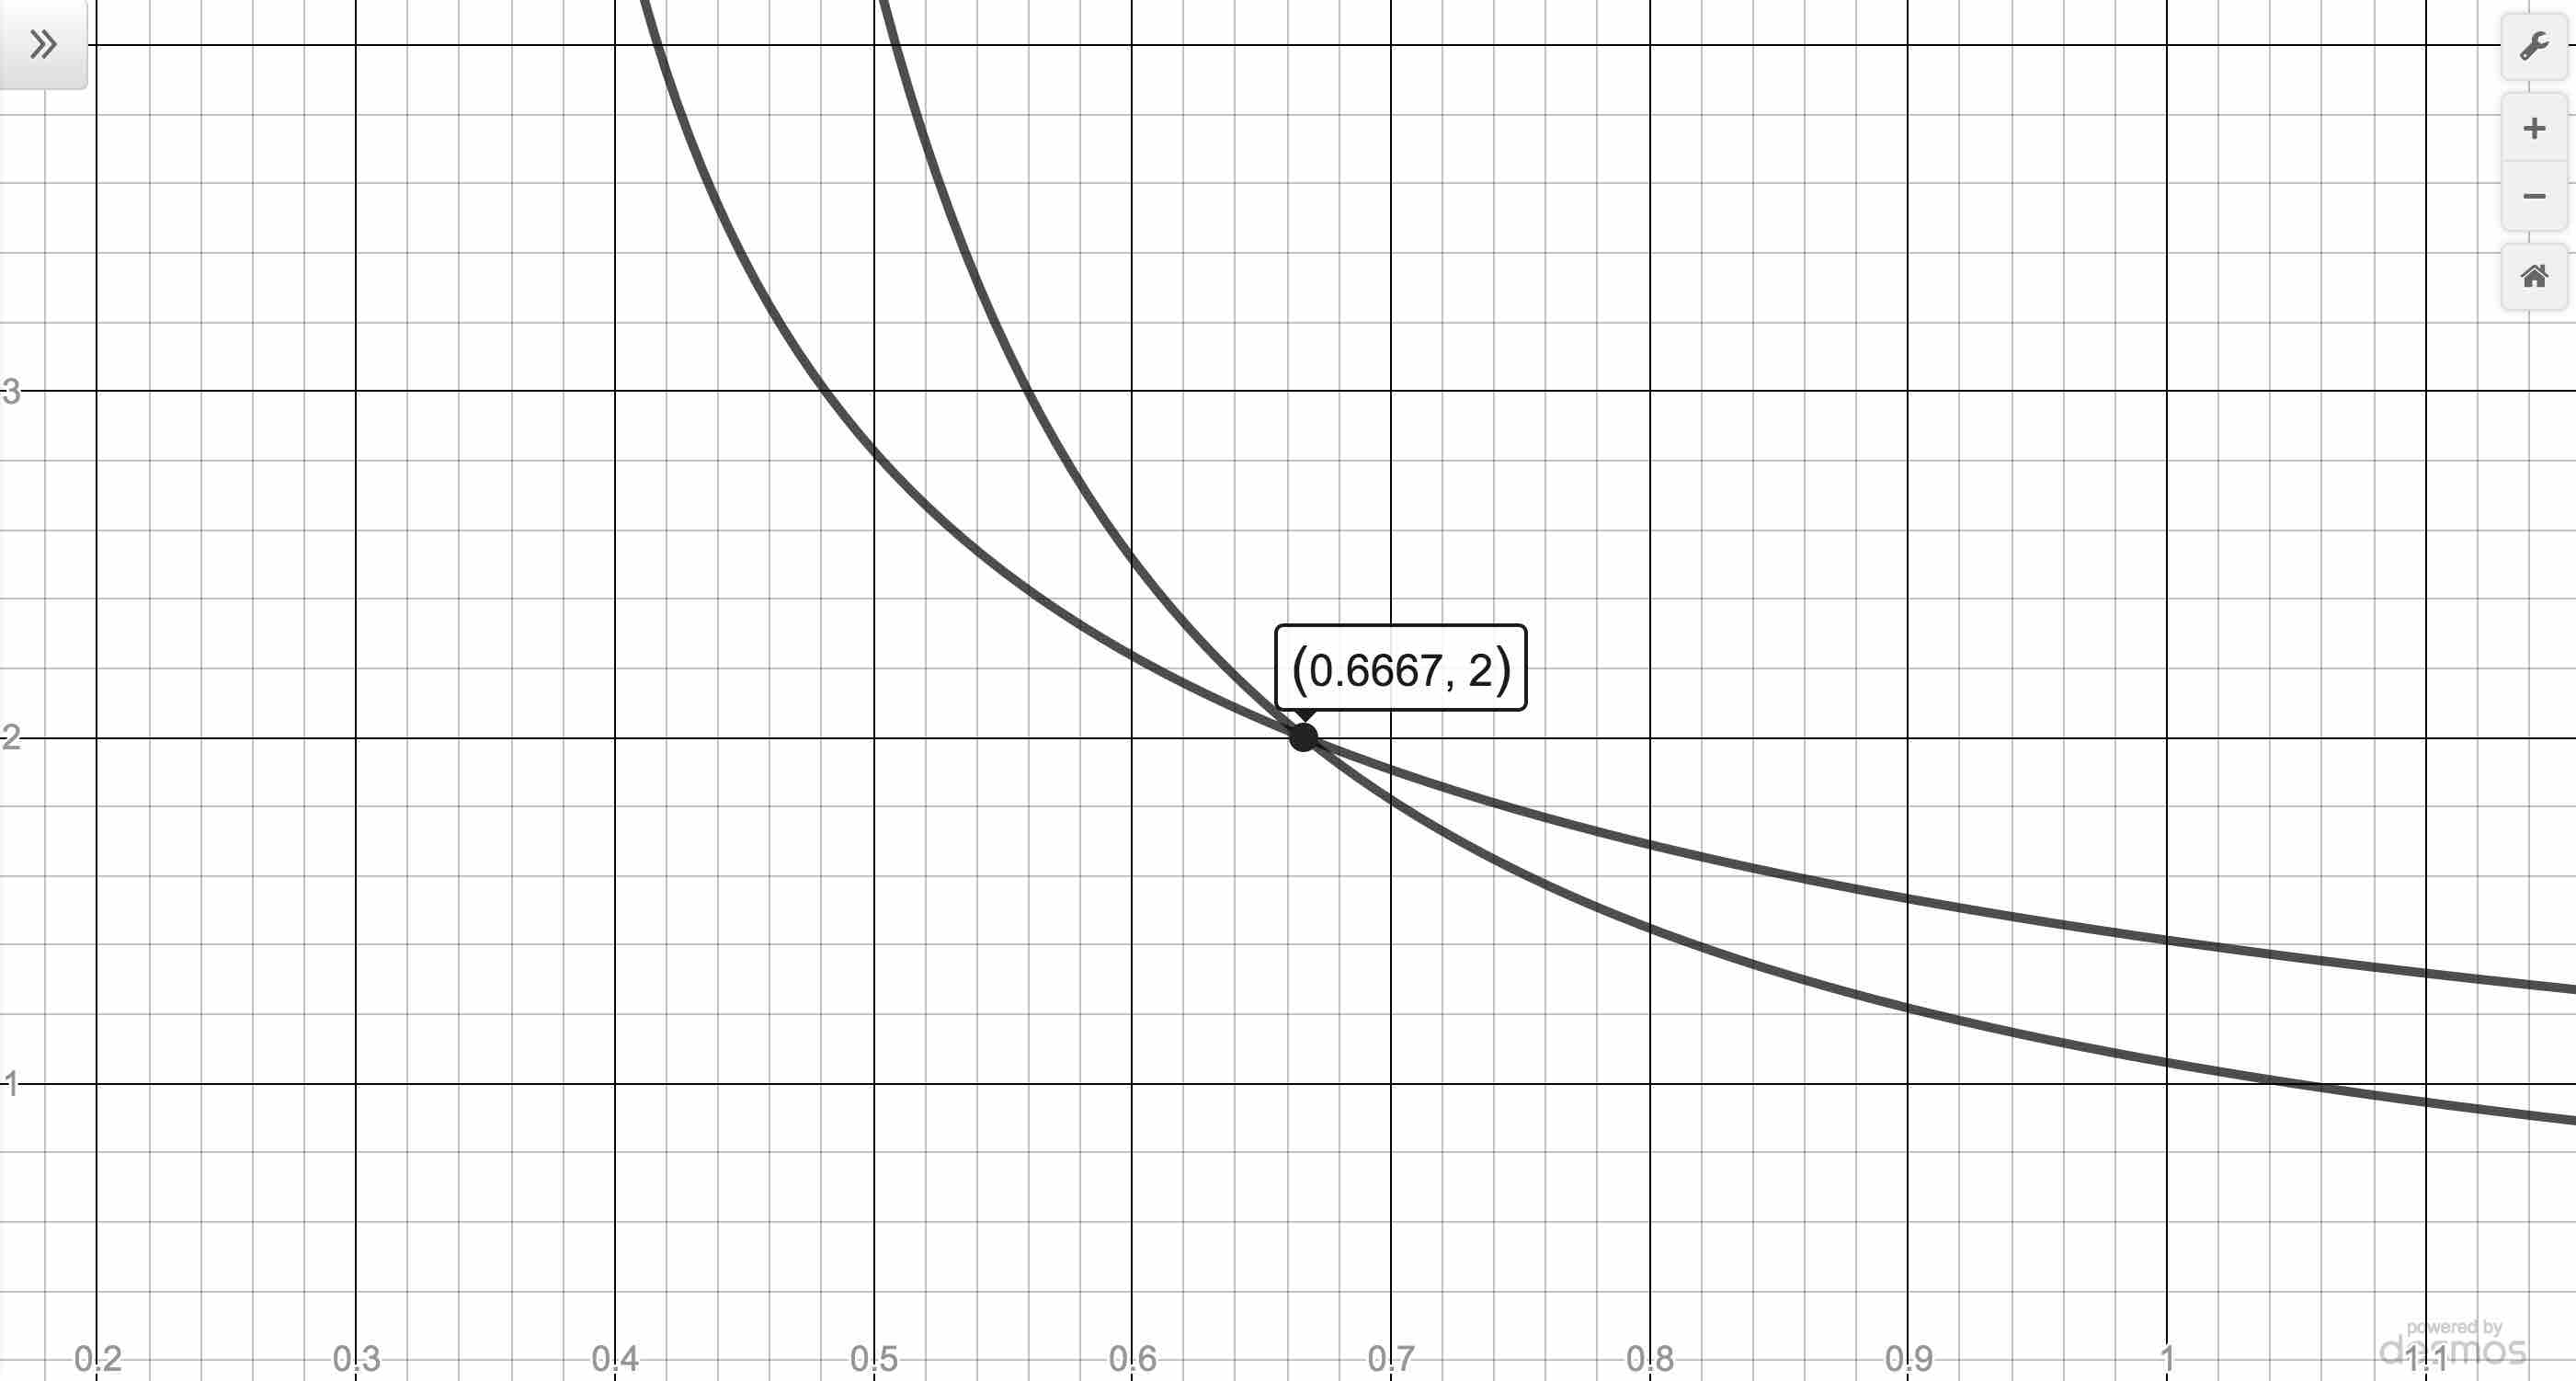
\includegraphics[width=3in]{./PowerEqIneqGraphics/PowerEqEx05.jpg} & 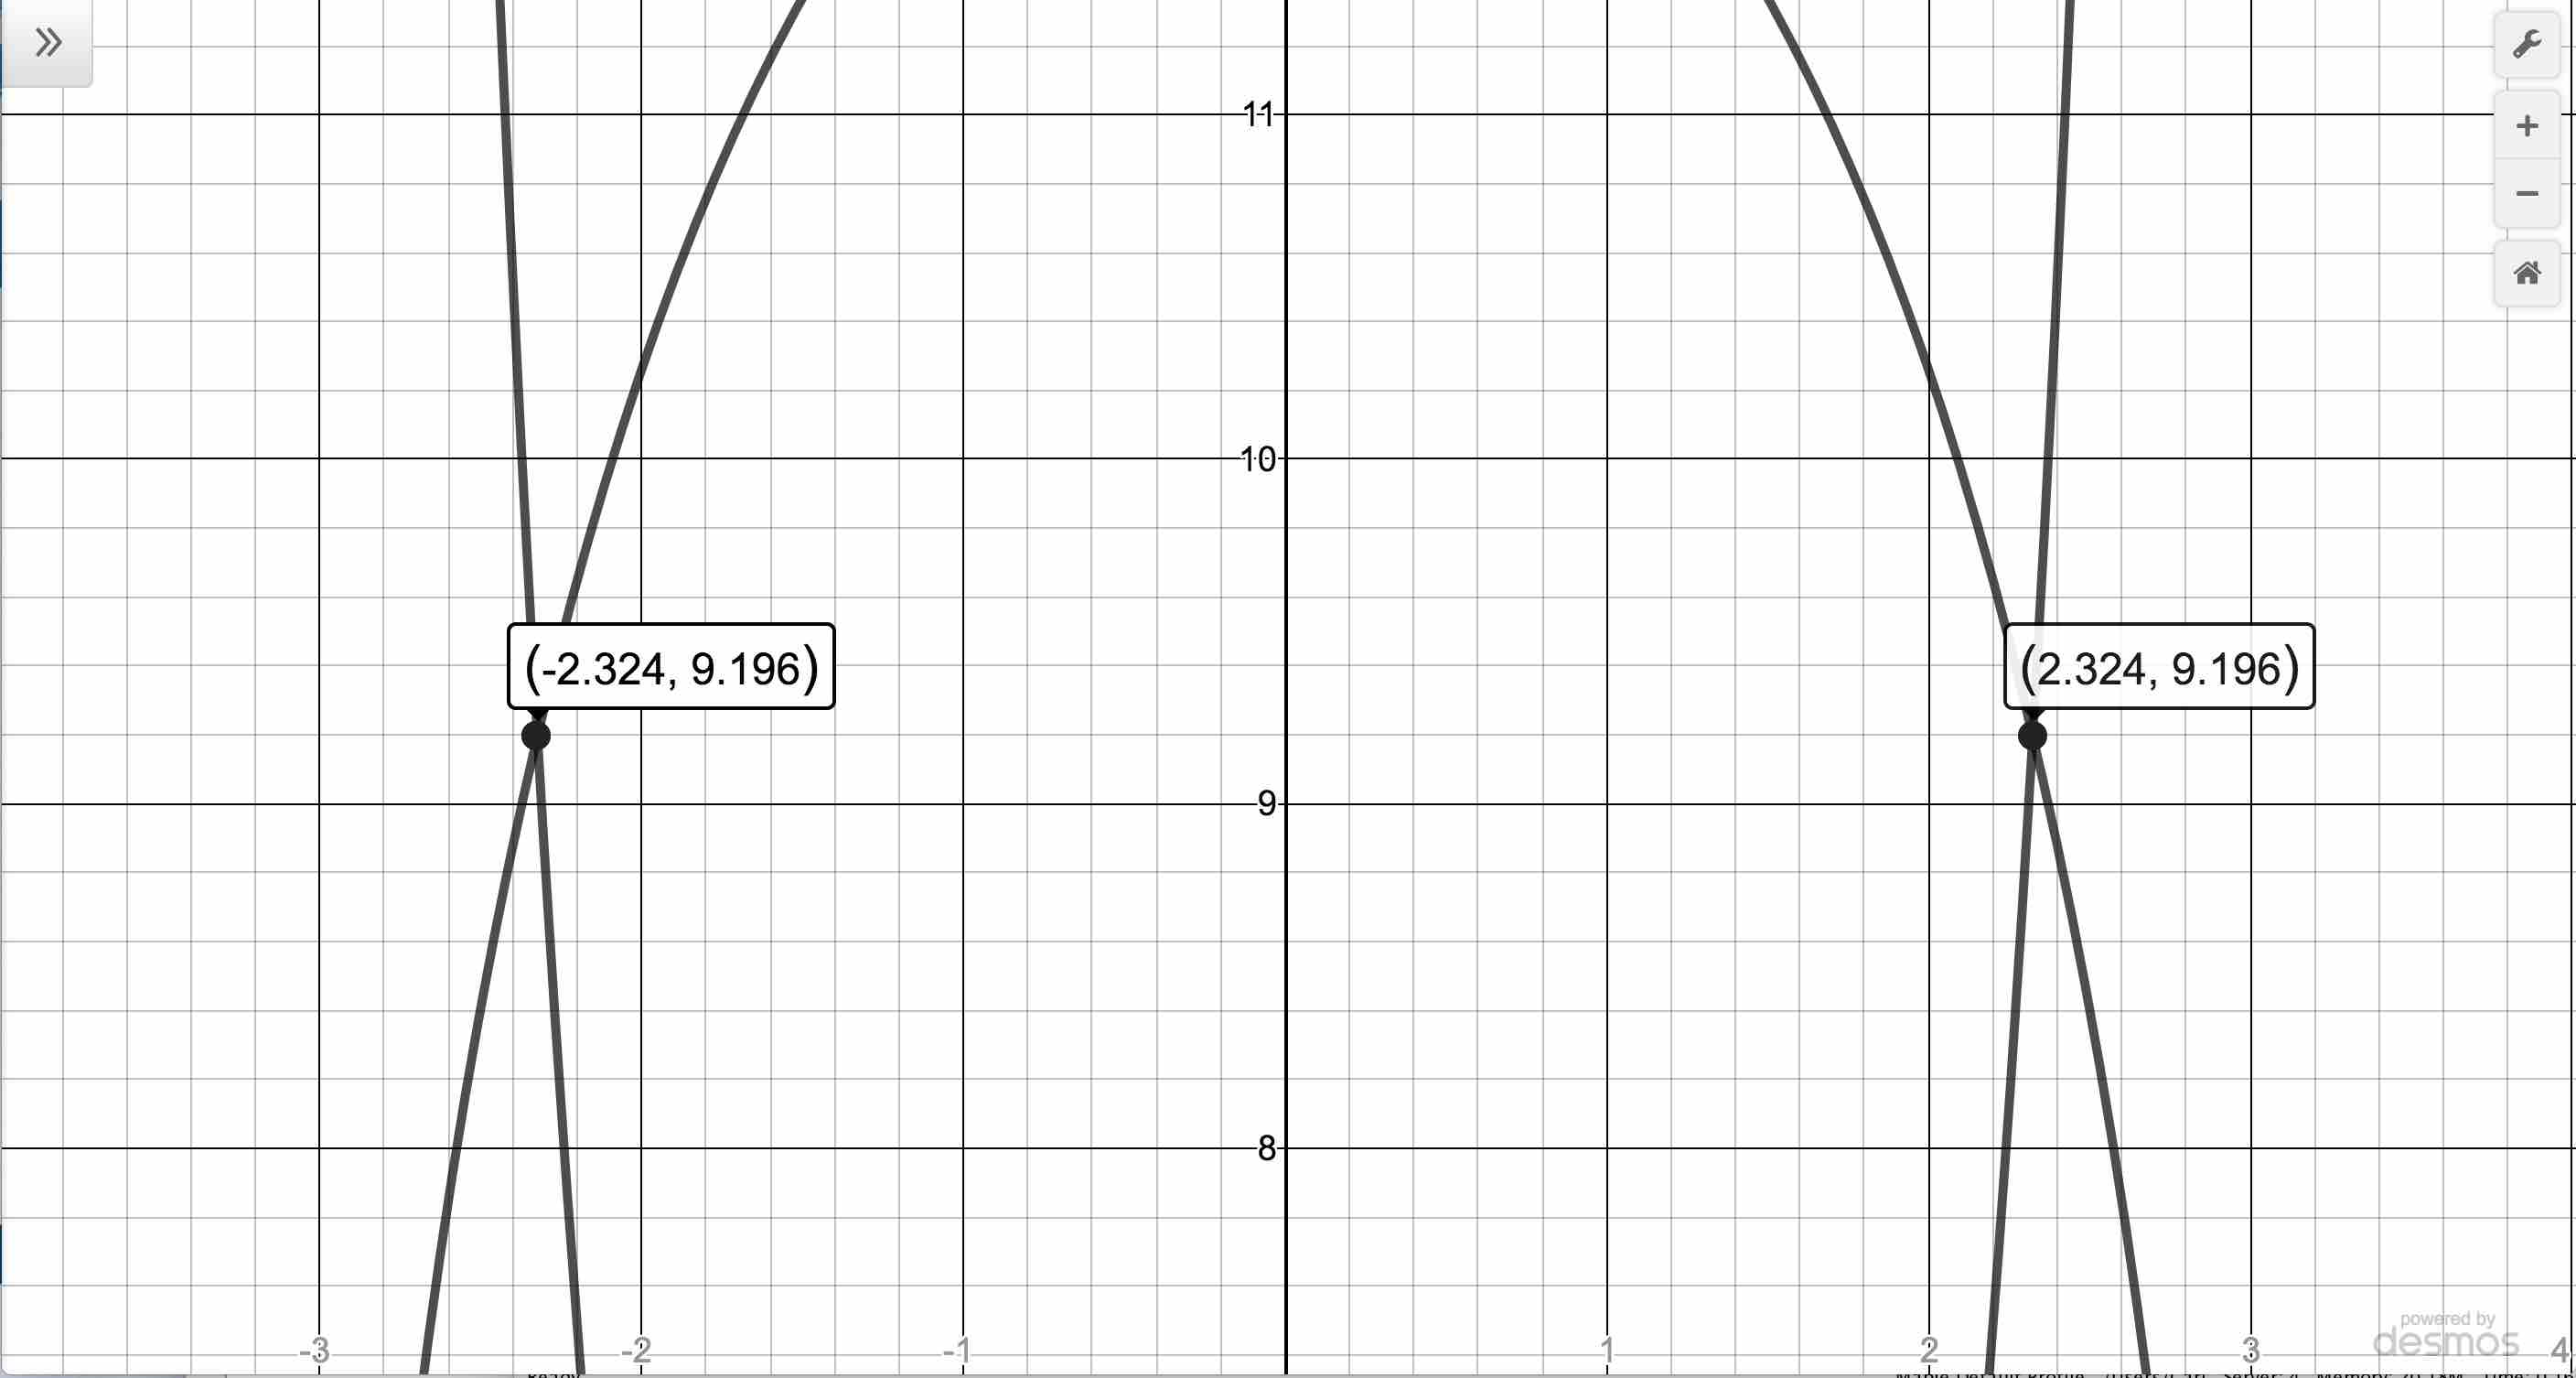
\includegraphics[width=3in]{./PowerEqIneqGraphics/PowerEqEx06.jpg} \\

Checking $2(3x-1)^{-0.5}  = 3x (3x-1)^{-1.5}$  & Checking  $6(9-t^2)^{\frac{1}{3}} = 4t^2 (9-x^2)^{\frac{2}{3}}$ \\

\end{tabular}

\end{center} 

\end{enumerate}

\qed

\end{ex}

Note that Example \ref{powerequationex}, there are several ways to correctly solve each equation, and we endeavored to demonstrate a variety of methods.  For example, for number \ref{first}, instead of converting $(7-x)^{\frac{3}{2}}$ to a radical equation, we could use Theorem \ref{exponentprops}.  Since the root here ($2$) is even, we know $7-x \geq 0$ or $x \leq 7$.  Hence we may apply exponent properties: 

\[ \begin{array}{rclr}  

(7-x)^{\frac{3}{2}} & = & 8 & \\

 \left[(7-x)^{\frac{3}{2}}\right]^{\frac{2}{3}} & = & 8^{\frac{2}{3}} & \text{raise both sides to the $\frac{2}{3}$ power} \\
 
 (7-x)^{\frac{3}{2} \cdot \frac{2}{3}} & = & 4 & \text{Theorem \ref{exponentprops}} \\
 
(7-x)^{1} & = & 4 \\ \end{array} \]

from which we get $x = 3$.  If we try this same approach to solve number \ref{second}, however, we encounter difficulty.  From $(2t-1)^{\frac{2}{3}} -4 = 0$, we get $(2t-1)^{\frac{2}{3}}  =4$.  

\[ \begin{array}{rclr}  

(2t-1)^{\frac{2}{3}} & = & 4 & \\

 \left[(2t-1)^{\frac{2}{3}}  \right]^{\frac{3}{2}} & = & 4^{\frac{3}{2}}& \text{raise both sides to the $\frac{3}{2}$ power} \\ \end{array} \]
 
 Since the root here ($3$) is odd, we have no restriction on $2t-1$ but the exponent $\frac{3}{2}$ has an even denominator.  Hence, Theorem \ref{exponentprops} \textit{does not apply}.  That is, \[\left[(2t-1)^{\frac{2}{3}}  \right]^{\frac{3}{2}} \neq (2t-1)^{\frac{2}{3} \cdot \frac{3}{2}} = (2t-1)^{1} = (2t-1).\]
 Note that if we weren't careful, we'd have $2t-1 = 4^{\frac{3}{2}} = 8$ which gives $t= \frac{9}{2} = 4.5$ only.   We'd have missed the solution $t = -3.5$.  Truth be told, you \textit{can} simplify $\left[(2t-1)^{\frac{2}{3}}  \right]^{\frac{3}{2}} $ - just not using Theorem \ref{exponentprops}.  We leave it as an exercise to show  $\left[(2t-1)^{\frac{2}{3}}  \right]^{\frac{3}{2}} = |2t-1|$ and, more generally, $\left(x^{\frac{2}{3}}\right)^{\frac{3}{2}} = |x|$.
 
 Our next example is an application of the  \href{https://en.wikipedia.org/wiki/Cobb-Douglas_production_function}{\underline{Cobb Douglas}} production model of an economy.  The Cobb-Douglas model states that the yearly total dollar value of the production output in an economy is a function of \textit{two} variables:   labor (the total number of hours worked in a year) and capital (the total dollar value of all of everything purchased in order to make things).  If we fix a certain production output level, this relates the labor to the capital - so knowing one allows us to know the other.   The formula relating the production output level $P$, labor $x$ and capital $y$ is $P = a x^{b} y^{1-b}$ where $a$, $x$, and $y$ are positive and $0 < b < 1$.    

\begin{ex} \label{CobbDouglasEx}  Suppose in a given economy, the Cobb-Douglas model is $500 = 1.5 x^{0.43} y^{0.57}$ where $x$ is measured in hundreds of thousands of hours of labor and $y$ is measured in millions of dollars.

\begin{enumerate}

\item  Find $y$ as a function of $x$:  $y = C(x)$.  

\item  Find and interpret $C(3)$.

\item Graph $y = C(x)$.  

\item Describe and interpret the behavior as $x \rightarrow 0^{+}$ and as $x \rightarrow \infty$.

\end{enumerate}


\end{ex}





\closegraphsfile